\documentclass[tikz,border=8pt]{standalone}
% Shared TikZ style for synorg platform diagrams. Each diagram \input's this
% inside a standalone document. Palette tracks the Material "teal" site theme so
% figures read as one system in light mode (SVGs are theme-neutral otherwise).
\usetikzlibrary{arrows.meta,positioning,shapes.geometric,fit,backgrounds,calc,decorations.pathreplacing}

\definecolor{synteal}{HTML}{00897B}   % primary
\definecolor{synfill}{HTML}{E0F2F1}   % light fill
\definecolor{synamber}{HTML}{B26A00}  % warning / lend
\definecolor{synred}{HTML}{B00020}    % deny / danger
\definecolor{syngrey}{HTML}{5F6368}   % muted

\tikzset{
  >=Stealth,
  font=\sffamily\small,
  box/.style={draw=synteal,line width=0.6pt,rounded corners=2pt,fill=synfill,
              inner sep=5pt,align=center},
  plane/.style={draw=synteal,line width=0.8pt,rounded corners=3pt,fill=synfill,
                inner sep=8pt,align=center},
  state/.style={draw=synteal,line width=0.7pt,circle,fill=synfill,inner sep=3pt,
                minimum size=11mm,align=center,font=\sffamily\footnotesize},
  decision/.style={draw=synteal,line width=0.7pt,diamond,aspect=2,fill=synfill,
                   inner sep=1pt,align=center,font=\sffamily\footnotesize},
  deny/.style={draw=synred,fill=synred!8,text=synred},
  warn/.style={draw=synamber,fill=synamber!10},
  flow/.style={->,line width=0.6pt,draw=syngrey},
  flowlbl/.style={font=\sffamily\footnotesize,text=syngrey,inner sep=2pt},
  note/.style={font=\sffamily\footnotesize\itshape,text=syngrey},
}

\begin{document}
% The agent operating loop (agent-interface.md): propose -> validate -> observe
% -> correct, closed by the agent alone with no human translator. Each stage
% names the repo surface it acts on.
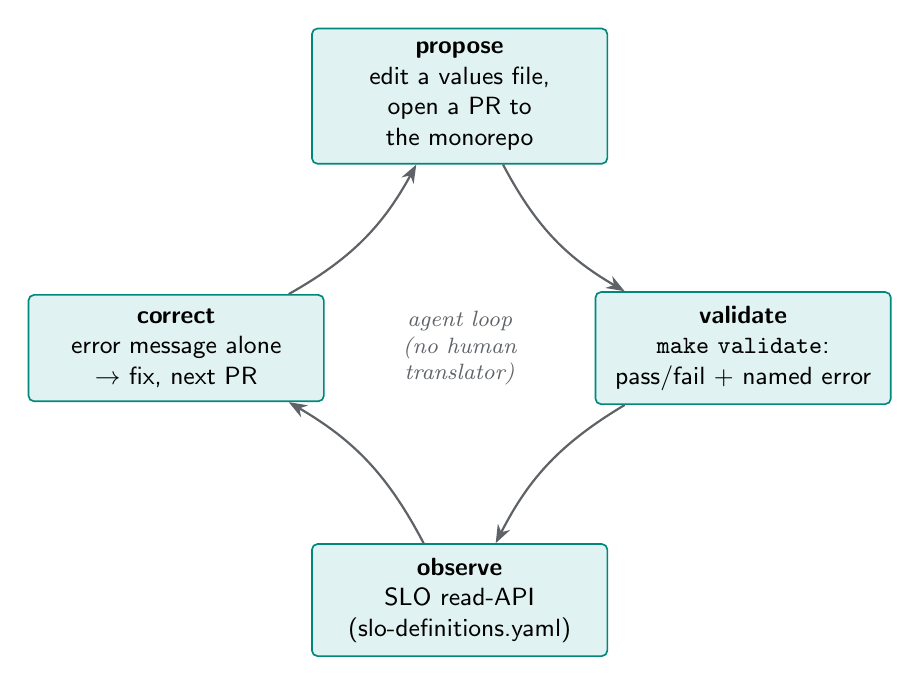
\begin{tikzpicture}
  \node[box,text width=34mm] (propose) at (90:3.2)
    {\textbf{propose}\\edit a values file,\\open a PR to the monorepo};
  \node[box,text width=34mm] (validate) at (0:3.6)
    {\textbf{validate}\\\texttt{make validate}:\\pass/fail + named error};
  \node[box,text width=34mm] (observe) at (-90:3.2)
    {\textbf{observe}\\SLO read-API\\(slo-definitions.yaml)};
  \node[box,text width=34mm] (correct) at (180:3.6)
    {\textbf{correct}\\error message alone\\$\to$ fix, next PR};

  \draw[flow,line width=0.8pt] (propose) to[bend right=16] (validate);
  \draw[flow,line width=0.8pt] (validate) to[bend right=16] (observe);
  \draw[flow,line width=0.8pt] (observe) to[bend right=16] (correct);
  \draw[flow,line width=0.8pt] (correct) to[bend right=16] (propose);

  \node[align=center,font=\footnotesize\itshape,text=syngrey] at (0,0)
    {agent loop\\(no human\\translator)};
\end{tikzpicture}
\end{document}
